\section{Method}
\label{sec:method}

\begin{figure}[t]
  \centering
  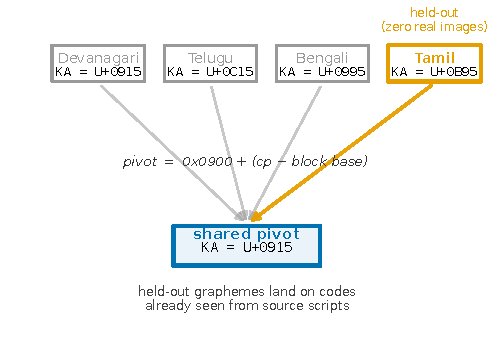
\includegraphics[width=\linewidth]{figs/fig1_pivot.pdf}
  \caption{The shared grapheme pivot space. Each Brahmic script maps bijectively into a common
  output space by ISCII-derived Unicode-offset correspondence (the same letter sits at the same
  offset within each block); grapheme clusters in that space form the recognizer's output
  vocabulary. A held-out script's graphemes therefore land on pivot codes already seen from the
  source scripts. The held-out script enters training only as verified synthetic renderings
  (Rung~B) or not at all (Rung~A); evaluation is always on its \emph{real} scene images.}
  \label{fig:method}
\end{figure}

\subsection{A shared grapheme pivot space for Brahmic scripts}
\label{sec:pivot}

Brahmic scripts encode the same phonological skeleton --- consonant bases, dependent vowel signs,
and conjunct formation through a virama --- and Unicode preserves this: corresponding letters sit
at the same offset within each script's block. We exploit both layers.

\paragraph{Structural pivot.} A mapping $\pi$ sends any Brahmic codepoint to a pivot codepoint by
its within-block offset ($\pi(c) = \mathrm{0x0900} + (c - \mathrm{base}(c))$); shared punctuation
that is not offset-safe is excluded by construction. Because $\pi$ is a per-script bijective
shift, it is exactly invertible: a hypothesis decoded in pivot space is read back into the target
script deterministically. Text from nine scripts thereby writes into one label space in which
structurally corresponding syllables become \emph{identical} strings.

\paragraph{Grapheme-cluster vocabulary.} Within pivot space we segment text into grapheme
clusters (consonant--virama conjuncts kept whole, dependent signs attached) and inject the
resulting cluster inventory (1{,}624 types for the source pool) as dedicated tokens into the
recognizer's tokenizer. The alternative --- letting the stock byte-BPE tokenizer segment
pivot-space text --- is the ablation of Sec.~\ref{sec:experiments}: it sees the same pivot
strings but fragments clusters into sub-syllabic pieces. Fertility (mean clusters per word)
governs when grapheme tokenization beats BPE in \emph{supervised} training: in a 12-run
balanced-budget study across the same nine scripts, fertility predicts the winning branch with
\lawPolarity\ polarity and $\lawLoso\%$ leave-one-script-out direction accuracy
($R^2\!=\!\lawRsqAdv$). % pointer to journal-length treatment; kept to motivation here
That result motivates both the pivot design and the (ultimately falsified) primary hypothesis of
Sec.~\ref{sec:analysis}.

\subsection{Zero-real-image protocol}
\label{sec:protocol}

For each held-out script $S$ of the nine in the benchmark~\cite{bstd}:

\noindent\textbf{Sources.} All benchmark languages whose script is not $S$ (languages sharing
$S$, e.g.\ Assamese for Bengali script, are excluded --- $S$ is genuinely unseen). Each source
language contributes exactly 700 train / 90 val real images (seed 42), giving balanced source
exposure by construction; source-side data size is therefore controlled, unlike prior
cross-lingual STR studies~\cite{crosslingstr}.

\noindent\textbf{Synthetic target.} 3{,}240 images per target language: benchmark-vocabulary
words rendered in fontconfig-verified fonts (multiple faces per script, libraqm shaping), each
render checked non-blank; the rendered word enters training as its pivot transcription. No real
photograph of $S$ is ever seen. Scripts written by two source languages receive two languages'
worth of renderings ($2\times$ budget) --- a covariate disclosed at preregistration time that
becomes central in Sec.~\ref{sec:analysis}.

\noindent\textbf{Rungs.} Rung~A trains on sources only; Rung~B adds the synthetic target set;
Rung~B$_{\mathrm{bpe}}$ repeats Rung~B with the grapheme-cluster injection removed (stock
tokenizer), identical data, seed, and recipe. All rungs fine-tune Florence-2
(0.23B)~\cite{florence2} with LoRA ($r\!=\!16$, $\alpha\!=\!32$, dropout 0.05), lr $10^{-4}$,
batch size 4, 15 epochs, validation-selected checkpoint, beam-search decoding at test.

\noindent\textbf{Evaluation.} The held-out script's real test split, WRR = exact match after NFC
normalization, zero-width-character removal, and whitespace collapse --- the benchmark's own
protocol~\cite{bstd,indicstr12} --- plus character accuracy ($1-\mathrm{CER}$).

\subsection{Preregistration and prospective predictions}
\label{sec:prereg}

The campaign ran under a frozen preregistration with an append-only amendment log; every
amendment was filed before the results it concerns existed. Descriptors entering the transfer
horse-race were computed result-blind: fertility and pivot coverage before any Rung-B result;
a frozen-encoder visual-similarity control before the third. Quantitative forecasts for later
runs were committed and pushed to a version-controlled archive \emph{before} those runs trained
(commit hashes in the supplementary material; archive anonymized for review), and are scored
against a rule fixed at filing time --- hits and misses alike (Sec.~\ref{sec:analysis}).
% Double-blind note: archive cited via anonymous mirror; hashes verifiable at camera-ready.
